\chapter{단일항, 벨 부등식, 그리고 복제 금지}

\lectureoverview{상대적인 마이너스 부호 하나가 단순히 상관된 두 스핀 상태를 회전 불변인 단일항 상태로 바꾼다. 전체 스핀을 계산해 그 상태를 확인하고, 완벽한 반상관성을 이용해 벨 실험을 구성한 다음, 고전적 명제를 양자 투영 연산자로 옮겨 표현한다. 그 결과 얻는 확률은 벨의 고전적 계수 세기 부등식을 위반한다. 국소성, 실험 시점, 불확정성에 관한 질문은 이어서 선형 양자역학의 두 번째 결과로 이어진다. 미지의 상태는 보편 복제기로 복사할 수 없다.}

\section{부호 하나가 무엇을 바꿀 수 있을까?}

전자 두 개를 생각하고 기저 상태에서는 텐서곱 기호를 생략하자:
\begin{equation}
  \ket{ud}\equiv\ket{u}_1\otimes\ket{d}_2,
  \qquad
  \ket{du}\equiv\ket{d}_1\otimes\ket{u}_2.
\end{equation}
특히 간단한 중첩 상태 두 개는 부호 하나만 다르다.
\begin{equation}
  \ket{\psi_\pm}
  =
  \frac{\ket{ud}\pm\ket{du}}{\sqrt2}.
  \label{eq:l05-two-signs}
\end{equation}
계수 \(1/\sqrt2\)는 전체 확률을 1로 만든다. 두 상태 모두에서 세 번째 축을 따라 측정하면 서로 반대인 결과가 나온다. 전자 1가 위쪽이면 전자 2는 아래쪽이고, 그 반대도 마찬가지다. 따라서 이 상관관계만으로는 부호를 알아낼 수 없다. 그런데도 두 상태는 물리적으로 서로 다르다.

계산에서는 파울리 연산자의 다음 작용을 반복해서 사용한다.
\begin{align}
  \sigma_1\ket{u}&=\ket{d},&
  \sigma_1\ket{d}&=\ket{u},\nonumber\\
  \sigma_2\ket{u}&=i\ket{d},&
  \sigma_2\ket{d}&=-i\ket{u},\nonumber\\
  \sigma_3\ket{u}&=\ket{u},&
  \sigma_3\ket{d}&=-\ket{d}.
  \label{eq:l05-pauli-actions}
\end{align}
전자 1에 작용하는 연산자에는 \(\sigma_i\)를 쓰고, 전자 2에 작용하는 동일한 연산자 집합은 \(\tau_i\)로 나타내자.

\begin{figure}[htbp]
\centering
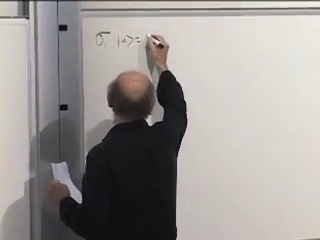
\includegraphics[width=0.62\linewidth]{lecture_05_figure_02.png}
\caption{비교 과정에서 사용하는 파울리 연산자의 전체 작용표.}
\lectureframe{00:03:15}
\end{figure}

두 상태 모두에서 어느 한쪽 스핀에도 선호되는 방향은 없다.
\begin{equation}
  \expect{\sigma_i}_{\psi_\pm}=0,
  \qquad
  \expect{\tau_i}_{\psi_\pm}=0,
  \qquad i=1,2,3.
  \label{eq:l05-local-zero}
\end{equation}
예를 들어, 요청된 플러스 상태의 명시적 계산은 다음과 같다.
\begin{align}
  \bra{\psi_+}\sigma_3\ket{\psi_+}
  &=
  \frac12
  \bigl(\bra{ud}+\bra{du}\bigr)
  \bigl(\ket{ud}-\ket{du}\bigr)\nonumber\\
  &=
  \frac12(1-1)=0.
  \label{eq:l05-sigma3-expectation}
\end{align}
\(\braket{ud}{du}=0\)이므로 교차항은 사라진다.

\begin{figure}[htbp]
\centering
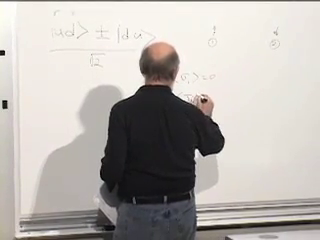
\includegraphics[width=0.78\linewidth]{lecture_05_figure_03.png}
\caption{플러스 상태의 기대값은 \(\sigma_3\)를 작용시키고 직교성을 이용해 계산한다.}
\lectureframe{00:07:00}
\end{figure}

\begin{classroomqa}
\lecturetimestamp{00:07:13}
\audiencequestion{기대값이 0이라는 것은 단일 스핀을 측정하면 값이 0으로 나온다는 뜻인가요?}
\lecturerresponse{아닙니다. 한 스핀 성분의 측정 결과는 \(+1\) 또는 \(-1\)뿐이며, \(\sigma_i\)에는 고윳값 0이 없습니다. 식~\eqref{eq:l05-local-zero}은 반복 측정 결과가 공정한 동전 던지기처럼 나온다는 뜻이지, 개별 측정 결과가 0이라는 뜻이 아닙니다.}
\end{classroomqa}

따라서 처음 생각해 볼 수 있는 진단 방법은 실패했다. 국소 평균으로는 상대 부호를 알 수 없으므로 두 입자쌍의 성질을 측정해야 한다.

\section{전체 스핀으로 단일항 상태를 판별하다}

입자쌍의 자기 모멘트는 벡터합으로 나타낸다.
\begin{equation}
  \boldsymbol{\Sigma}
  =
  \boldsymbol{\sigma}+\boldsymbol{\tau}.
\end{equation}
그 세 번째 성분은 두 기저 벡터 모두를 영벡터로 보낸다.
\begin{align}
  (\sigma_3+\tau_3)\ket{ud}
  &=(1-1)\ket{ud}=0,\nonumber\\
  (\sigma_3+\tau_3)\ket{du}
  &=(-1+1)\ket{du}=0.
\end{align}
따라서
\begin{equation}
  (\sigma_3+\tau_3)\ket{\psi_\pm}=0.
\end{equation}
어느 부호를 택하든 모든 시행에서 전체 세 번째 성분은 0이다.

첫 번째 성분은 두 상태를 구별한다. 식~\eqref{eq:l05-pauli-actions}에서,
\begin{align}
  (\sigma_1+\tau_1)\ket{ud}
  &=\ket{dd}+\ket{uu},\nonumber\\
  (\sigma_1+\tau_1)\ket{du}
  &=\ket{uu}+\ket{dd}.
\end{align}
따라서
\begin{align}
  (\sigma_1+\tau_1)\ket{\psi_+}
  &=
  \sqrt2\bigl(\ket{uu}+\ket{dd}\bigr),\nonumber\\
  (\sigma_1+\tau_1)\ket{\psi_-}
  &=0.
  \label{eq:l05-total-x}
\end{align}
플러스 상태에서 이 관측량의 기대값은 0일 수 있지만, 이 상태가 고윳값 0에 대응하는 고유상태인 것은 아니다.

\begin{classroomqa}
\lecturetimestamp{00:13:02}
\audiencequestion{전체 성분이 상태를 영벡터로 보내지 않을 때는 어떤 측정 결과가 가능한가요?}
\lecturerresponse{각 입자의 측정 결과는 \(+1\) 또는 \(-1\)이므로, 두 결과의 합은 \(2\), \(0\) 또는 \(-2\)일 수 있습니다. 기대값이 0이라고 해서 모든 시행에서 결과가 0인 것은 아닙니다.}
\end{classroomqa}

두 번째 성분을 확인하면 검증이 완성된다. 반대칭 조합에서는 \(i\)의 인자들이 상쇄된다.
\begin{equation}
  (\sigma_2+\tau_2)\ket{\psi_-}=0.
\end{equation}
따라서 세 성분 모두 마이너스 상태를 영벡터로 보낸다.
\begin{equation}
  \bigl(\boldsymbol{\sigma}+\boldsymbol{\tau}\bigr)
  \cdot\hat n\,\ket{\psi_-}=0
  \qquad\text{for every unit vector }\hat n.
  \label{eq:l05-singlet-any-axis}
\end{equation}

\begin{figure}[htbp]
\centering
\includegraphics[width=0.84\linewidth]{lecture_05_figure_06.png}
\caption{마이너스 상태의 전체 스핀이 0임을 보여 주는 성분별 상쇄.}
\lectureframe{00:16:30}
\end{figure}

반대칭 상태 \(\ket{\psi_-}\)는 \emph{단일항}이다. 이 상태는 회전 불변이다. 어느 축을 택해도 전체 스핀의 측정 결과는 0이다. 식~\eqref{eq:l05-two-signs}에 나오는 대칭 상태는 삼중항 부문에 속한다.

\begin{classroomqa}
\lecturetimestamp{00:19:06}
\audiencequestion{서로 반대인 스핀 결과는 평균적으로만 성립하나요?}
\lecturerresponse{단일항 상태에서는 모든 시행에서 성립합니다. 식~\eqref{eq:l05-singlet-any-axis}은 고유벡터 방정식이므로 두 입자에서 같은 성분을 측정하면 언제나 그 합이 고윳값 0인 결과를 얻습니다.}
\end{classroomqa}

\begin{classroomqa}
\lecturetimestamp{00:19:36}
\audiencequestion{다른 상태는 왜 삼중항이라고 부르나요?}
\lecturerresponse{그 이름은 전체 스핀 1 다중항에 속하는 세 상태에서 왔습니다. 유도는 나중으로 미루고, 여기서는 대칭 상태와 1차원 단일항 부문의 차이만 살펴보겠습니다.}
\end{classroomqa}

밥이 전자에서 임의의 성분을 측정하면, 앨리스가 자기 전자에서 같은 성분을 측정했을 때 어떤 결과를 얻을지 바로 알 수 있다. 앨리스의 결과는 반드시 그 반대다. 이것이 아인슈타인--포돌스키--로젠 상관관계다. 숨은 결과가 서로 반대인 동전 두 개도 있을 수 있지만, 미리 정해 둔 질문 하나에 대해서만 그렇다. 단일항 상태에서는 어떤 공간축을 선택하든 완벽한 반상관성이 성립한다.

\begin{classroomqa}
\lecturetimestamp{00:20:55}
\audiencequestion{얽힘을 처음 발견한 사람은 아인슈타인, 포돌스키, 로젠인가요?}
\lecturerresponse{아닙니다. 슈뢰딩거가 이 현상을 논의하고 얽힘이라는 용어를 도입했습니다. EPR 논증은 멀리 떨어진 입자 사이의 상관관계 문제를 특히 선명하게 드러냈습니다.}
\end{classroomqa}

\begin{classroomqa}
\lecturetimestamp{00:23:50}
\audiencequestion{즉각적인 상관관계는 인과율에 어긋나나요? 어느 관찰자가 먼저 측정하는지가 중요한가요?}
\lecturerresponse{전달할 수 있는 신호는 없습니다. 밥이 측정했는지와 관계없이, 어떤 관성계에서 보더라도 앨리스의 국소 측정 결과는 각각 절반의 확률로 나온다. 앨리스가 상관관계를 확인하려면 밥의 결과를 보통의 고전적 통신 채널로 전달받아야 하며, 그 신호는 빛보다 빠를 수 없다.}
\end{classroomqa}

\section{벨 부등식은 고전적인 계수 부등식이다}

벨의 결과가 무엇을 뜻하는지는 때로 분명하지 않게 느껴진다. 어떤 때는 양자역학의 가장 깊은 특징처럼 보이고, 다른 때는 형식론에서 필연적으로 따라 나오는 결과 중 하나처럼 보인다. 벨 자신도 파인먼도 이 두 관점을 모두 표현할 수 있었다. 하지만 부등식 자체는 기초적이다. 놀라운 점은 그것이 위반된다는 사실이다.

보통의 물체 집합을 생각해 보자. 각 물체는 세 성질 \(A\), \(B\), \(C\)을 가질 수도 있고 갖지 않을 수도 있다. \(N(A,\neg B)\)는 \(A\)은 가지지만 \(B\)은 갖지 않는 물체의 수를 나타내자. 고전적 집합 논리로부터 다음이 성립한다.
\begin{equation}
  N(A,\neg B)+N(B,\neg C)
  \geq
  N(A,\neg C).
  \label{eq:l05-bell-count}
\end{equation}
증명은 다음 집합 포함 관계에 따른다.
\begin{equation}
  A\cap C^{c}
  \subseteq
  (A\cap B^{c})\cup(B\cap C^{c}).
  \label{eq:l05-set-inclusion}
\end{equation}
실제로 \(A\cap C^c\)의 원소는 \(B\)에 속하거나 속하지 않는다. 첫 번째 경우에는 \(B\cap C^c\)에 속하고, 두 번째 경우에는 \(A\cap B^c\)에 속한다. 합집합의 원소 수를 세면 왼쪽 집합의 원소 수보다 많아질 수는 있어도 적어지지는 않는다.

\begin{figure}[htbp]
\centering
\includegraphics[width=0.78\linewidth]{lecture_05_figure_07.png}
\caption{칠판 위의 증명은 서로 겹치는 세 고전적 부분집합을 음이 아닌 영역들로 나눈다.}
\lectureframe{00:31:15}
\end{figure}

달리 말해, 세 집합 도형의 서로 겹치지 않는 영역에 음이 아닌 정수 \(N_i\)를 붙이자. 식~\eqref{eq:l05-bell-count}의 양변에는 \(A\cap C^c\)에 필요한 영역이 모두 포함되고, 왼쪽에는 음이 아닌 영역이 추가로 들어간다. 양자적인 내용은 전혀 개입하지 않는다. 이는 부분집합과 일반적인 논리적 선택지에 관한 정리다.

\section{집합 명제를 스핀 실험으로 옮기기}

많은 전자쌍을 서로 독립적으로 준비해 단일항 상태에 두고, 전자 1에 관해 다음 세 명제를 정의하자.
\begin{align}
  A&:\ \text{spin 1 is up at }0^\circ\text{, along the third axis},\nonumber\\
  B&:\ \text{spin 1 is up at }45^\circ\text{ in the }zx\text{-plane},\nonumber\\
  C&:\ \text{spin 1 is up at }90^\circ\text{, along the first axis}.
  \label{eq:l05-abc}
\end{align}

\begin{figure}[htbp]
\centering
\includegraphics[width=0.82\linewidth]{lecture_05_figure_08.png}
\caption{세 스핀 명제는 한 평면 안의 \(0^\circ\), \(45^\circ\), \(90^\circ\) 방향으로 정해져 있다.}
\lectureframe{00:39:00}
\end{figure}

단일항 상태에서는 전자 1에 관한 명제의 부정을 전자 2에 관한 긍정 명제로 바꿔 쓸 수 있다. 예를 들어,
\begin{align}
  \neg B
  &:\ \text{spin 1 is down at }45^\circ\nonumber\\
  &\Longleftrightarrow
  \text{spin 2 is up at }45^\circ.
\end{align}
마찬가지로 \(\neg C\)은 전자 2가 \(90^\circ\) 방향에서 위쪽이라는 명제가 된다.

\begin{classroomqa}
\lecturetimestamp{00:40:04}
\audiencequestion{\(\neg C\)는 전자 2가 \(90^\circ\) 방향에서 아래쪽임을 뜻하나요?}
\lecturerresponse{아닙니다. 먼저 \(C\)를 부정하면 전자 1는 \(90^\circ\) 방향에서 아래쪽입니다. 단일항 상태의 완벽한 반상관성에 따라 전자 2는 같은 축을 따라 위쪽이 됩니다. 이 두 번의 반전을 구분해야 합니다.}
\end{classroomqa}

계가 충분히 크면 계수와 확률의 차이는 준비된 쌍의 공통 개수뿐이다. 회전 불변성으로부터 다음도 성립한다.
\begin{equation}
  P(A,\neg B)=P(B,\neg C),
\end{equation}
두 번째 실험은 첫 번째 실험을 \(45^\circ\)만큼 회전한 것이기 때문이다. 따라서 벨의 고전적 부등식은 다음을 요구한다.
\begin{equation}
  2P(A,\neg B)\geq P(A,\neg C).
  \label{eq:l05-bell-probability}
\end{equation}
이제 이 확률들을 효율적으로 계산할 방법이 필요하다.

\section{명제를 투영 연산자로 나타내기}

보통의 3차원 벡터 공간에서 투영 연산자는 선택한 부분공간에 수직인 성분을 모두 제거한다. 1차원 투영 연산자는 벡터를 직선에 직교 투영하고, 2차원 투영 연산자는 평면에 직교 투영한다. \(P\)가 특정 부분공간으로의 투영 연산자라면,
\begin{equation}
  P\ket{\alpha}=\ket{\alpha_P}.
\end{equation}

\begin{figure}[htbp]
\centering
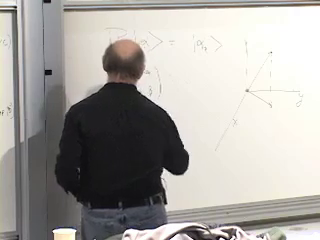
\includegraphics[width=0.76\linewidth]{lecture_05_figure_04.png}
\caption{기하학적 투영과 그 연산자 표기를 나란히 살펴본다.}
\lectureframe{00:49:53}
\end{figure}

\begin{figure}[htbp]
\centering
\begin{tikzpicture}[scale=1.05,>=Latex]
  \draw[->] (-0.25,0)--(4.0,0);
  \draw[thick] (-0.25,-0.25)--(3.55,2.6);
  \draw[->,very thick] (0,0)--(2.25,3.05)
    node[above] {\(\ket{\alpha}\)};
  \coordinate (P) at (2.72,1.98);
  \draw[dashed] (2.25,3.05)--(P);
  \draw[->,very thick] (0,0)--(P)
    node[right] {\(\ket{\alpha_P}\)};
  \node[below right] at (3.1,2.25) {projected subspace};
\end{tikzpicture}
\caption{투영 기하를 명확하게 다시 구성한 그림.}
\end{figure}

한 스핀의 힐베르트 공간에서 \(\sigma_3=+1\)이라는 명제는 \(\ket{u}\)가 생성하는 1차원 부분공간에 대응한다. 그 투영 연산자의 작용은 다음과 같다.
\begin{equation}
  P_{\sigma_3=+1}
  \begin{pmatrix}\alpha\\\beta\end{pmatrix}
  =
  \begin{pmatrix}\alpha\\0\end{pmatrix},
  \qquad
  P_{\sigma_3=-1}
  \begin{pmatrix}\alpha\\\beta\end{pmatrix}
  =
  \begin{pmatrix}0\\\beta\end{pmatrix}.
  \label{eq:l05-projector-actions}
\end{equation}

\begin{classroomqa}
\lecturetimestamp{00:49:55}
\audiencequestion{첫 번째 투영 연산자는 벡터가 수직축에서 얼마나 높은지 나타내나요?}
\lecturerresponse{아닙니다. 직교 성분인 \(\beta\)만 버립니다. 성분들은 힐베르트 공간의 진폭이지, 스핀의 보통 공간 좌표가 아닙니다.}
\end{classroomqa}

\begin{figure}[htbp]
\centering
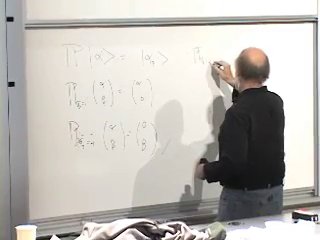
\includegraphics[width=0.78\linewidth]{lecture_05_figure_05.png}
\caption{투영 연산자를 먼저 일반적인 스피너에 작용시킨 다음 명시적인 행렬로 나타낸다.}
\lectureframe{00:51:40}
\end{figure}

행렬 형태는 다음과 같다.
\begin{equation}
  P_{\sigma_3=+1}
  =
  \begin{pmatrix}1&0\\0&0\end{pmatrix}
  =
  \frac{I+\sigma_3}{2}.
  \label{eq:l05-p3}
\end{equation}
같은 구성은 임의의 단위벡터 \(\hat n\) 방향에도 적용된다.
\begin{equation}
  P_{\boldsymbol{\sigma}\cdot\hat n=+1}
  =
  \frac{I+\boldsymbol{\sigma}\cdot\hat n}{2}.
  \label{eq:l05-pn}
\end{equation}

\begin{classroomqa}
\lecturetimestamp{00:53:09}
\audiencequestion{\(\sigma_1=+1\)에 대한 투영 연산자는 무엇인가요?}
\lecturerresponse{식~\eqref{eq:l05-p3}에서 \(\sigma_3\)를 \(\sigma_1\)로 바꾸면 됩니다. 즉, \(P_{\sigma_1=+1}=(I+\sigma_1)/2\)입니다.}
\end{classroomqa}

이제 보른 규칙을 명제의 형태로 유용하게 쓸 수 있다.
\begin{equation}
  P(\mathcal A\text{ is true in }\ket{\psi})
  =
  \bra{\psi}P_{\mathcal A}\ket{\psi}.
  \label{eq:l05-projector-born}
\end{equation}
정규화된 스피너 \(\ket{\psi}=(\alpha,\beta)^T\)에 대해 식~\eqref{eq:l05-projector-born}에서 \(P_{\sigma_3=+1}\)를 택하면 \(|\alpha|^2\)을 얻으며, 이는 예상한 결과다.

이 표현을 통해 고전적 명제와 양자 명제의 차이가 드러난다. 고전 논리에서 성질은 집합의 부분집합에 대응한다. 양자역학에서 성질은 힐베르트 공간의 부분공간, 또는 그에 대응하는 투영 연산자에 해당한다. 부분집합과 벡터 부분공간은 같은 격 연산을 따르지 않는다. 벨의 모순은 바로 그 차이에서 비롯된다.

\subsection{벨의 공동 투영 연산자}

\(A\wedge\neg B\)의 경우, 전자 1는 세 번째 축 방향으로 위쪽이어야 하고 전자 2는 다음 방향을 따라 위쪽이어야 한다.
\begin{equation}
  \hat n_{45}=\frac{\hat x+\hat z}{\sqrt2}.
\end{equation}
두 번째 스핀의 해당 성분은 다음과 같다.
\begin{equation}
  \boldsymbol{\tau}\cdot\hat n_{45}
  =
  \frac{\tau_1+\tau_3}{\sqrt2}.
\end{equation}
따라서 공동 투영 연산자는 다음과 같다.
\begin{equation}
  P_{A\wedge\neg B}
  =
  \frac{I+\sigma_3}{2}
  \frac{I+(\tau_1+\tau_3)/\sqrt2}{2}.
  \label{eq:l05-joint-projector}
\end{equation}

\begin{classroomqa}
\lecturetimestamp{00:59:18}
\audiencequestion{\(1/\sqrt2\)라는 계수가 \(45^\circ\) 스핀 성분에 들어가는 이유는 무엇인가요?}
\lecturerresponse{방향 벡터는 단위벡터여야 합니다. 첫 번째 축과 세 번째 축 방향의 성분이 모두 \(1/\sqrt2\)이므로, 이에 대응하는 관측량은 \((\tau_1+\tau_3)/\sqrt2\)입니다.}
\end{classroomqa}

\begin{classroomqa}
\lecturetimestamp{01:00:52}
\audiencequestion{식 전체 \(I+\boldsymbol{\tau}\cdot\hat n_{45}\)을 2로 나누나요?}
\lecturerresponse{네. 투영 연산자는 \(\bigl(I+\boldsymbol{\tau}\cdot\hat n_{45}\bigr)/2\)이며, 계수 \(1/2\)는 분자 전체에 곱해집니다.}
\end{classroomqa}

식~\eqref{eq:l05-joint-projector}의 두 인자는 서로 다른 텐서 인자에 작용하므로 서로 교환한다. 두 인자를 차례로 적용하면 먼저 전자 1가 아래쪽인 성분을 모두 제거하고, 남은 성분 가운데 전자 2가 \(\hat n_{45}\) 방향에서 아래쪽인 성분을 제거한다.

\section{양자수는 부등호의 방향을 뒤집는다}

다음을
\begin{equation}
  \ket{\psi_s}
  =
  \frac{\ket{ud}-\ket{du}}{\sqrt2}
\end{equation}
단일항 상태라 하자. 먼저 다음 식에서 시작한다.
\begin{equation}
  P(A,\neg B)
  =
  \bra{\psi_s}P_{A\wedge\neg B}\ket{\psi_s}.
\end{equation}
인자 \((I+\sigma_3)/2\)는 \(\ket{du}\)을 없애고 \(\ket{ud}/\sqrt2\)만 남긴다. 이어서 두 번째 인자를 적용하면
\begin{align}
  \frac{I+(\tau_1+\tau_3)/\sqrt2}{2}\ket{ud}
  &\notag\\[-0.3em]
  &=
  \frac12
  \left[
    \ket{ud}
    +\frac{\ket{uu}-\ket{ud}}{\sqrt2}
  \right]\nonumber\\
  &=
  \frac12
  \Biggl[
    \left(1-\frac1{\sqrt2}\right)\ket{ud}
  \nonumber\\
  &\qquad
    +\frac1{\sqrt2}\ket{uu}\Biggr].
  \label{eq:l05-projector-action}
\end{align}
\(\ket{uu}\)항은 단일항 브라와의 내적이 0이고, 남는 정규화 인자들을 계산하면 다음을 얻는다.
\begin{equation}
  P(A,\neg B)
  =
  \frac14\left(1-\frac1{\sqrt2}\right).
  \label{eq:l05-pab}
\end{equation}

\begin{figure}[htbp]
\centering
\includegraphics[width=0.88\linewidth]{lecture_05_figure_09.png}
\caption{투영 연산자 계산에서는 \(\ket{ud}\)와 겹치는 성분을 남기고 직교하는 \(\ket{uu}\) 성분을 제거한다.}
\lectureframe{01:08:20}
\end{figure}

회전 불변성에 따라 다음 두 방향에서도 같은 결과를 얻는다.
\begin{equation}
  P(B,\neg C)
  =
  \frac14\left(1-\frac1{\sqrt2}\right).
\end{equation}
\(A\wedge\neg C\)의 경우 두 번째 축이 첫 번째 공간축과 같으므로,
\begin{equation}
  P_{A\wedge\neg C}
  =
  \frac{I+\sigma_3}{2}\frac{I+\tau_1}{2}.
\end{equation}
첫 번째 인자는 다시 \(\ket{ud}/\sqrt2\)만 남긴다. \(\tau_1\) 항은 \(\ket{uu}\)를 만들며, 이는 단일항 브라와 직교한다. 반면 항등 연산자 항은 살아남는다. 따라서
\begin{equation}
  P(A,\neg C)=\frac14.
  \label{eq:l05-pac}
\end{equation}
세 결과를 합치면,
\begin{equation}
  \underbrace{
  P(A,\neg B)+P(B,\neg C)
  }_{\frac12(1-1/\sqrt2)\approx0.146}
  <
  \underbrace{
  P(A,\neg C)
  }_{\frac14=0.25}.
  \label{eq:l05-bell-violation}
\end{equation}

\begin{figure}[htbp]
\centering
\includegraphics[width=0.84\linewidth]{lecture_05_figure_10.png}
\caption{완성된 칠판 계산은 벨 부등식의 왼쪽 값이 더 작고 오른쪽 값이 더 큼을 보여 준다.}
\lectureframe{01:12:15}
\end{figure}

식~\eqref{eq:l05-bell-violation}은 식~\eqref{eq:l05-bell-probability}을 뒤집는다. 그렇다고 양자역학이 자기모순이라는 뜻은 아니다. 단일항 상관관계는 세 스핀 명제 모두가 먼 곳의 측정 선택과 무관하게 통상적인 집합론적 참·거짓 값을 가진다고 보는 국소적 고전 모형으로는 설명할 수 없다. 고전적 모형으로 이 상관관계를 재현하려면 벨 가정 가운데 적어도 하나를 포기해야 하며, 가장 두드러진 가정은 국소성이다.

\section{벨 실험이 검증하는 것}

양자역학은 이미 부등식 위반을 예측한다. 여기에 더해 실험에서는 한 검출기가 상대편 검출기에 자신이 만난 설정이나 결과를 알려 주는 고전적 우회 경로를 차단해야 한다. 두 측정 장치는 충분히 멀리 떨어져 있어야 하며, 측정 설정의 선택과 검출 시점은 빛의 속도로도 장치 사이를 오갈 수 없을 만큼 가까운 시간 간격 안에 있어야 한다. 아스페의 실험은 그러한 시간 조건과 분리를 실질적으로 납득할 수 있게 했다.

\begin{classroomqa}
\lecturetimestamp{01:13:15}
\audiencequestion{양자역학이 이미 답을 준다면 벨 실험은 무엇을 밝혔나요?}
\lecturerresponse{자연이 바로 이 상관관계 실험에서 양자역학의 예측을 따르는지 검증했고, 특히 두 측정 장치가 관련된 빛의 이동 시간 동안 서로 독립적으로 작동하도록 했습니다. 실험 제어와 시간 조정 자체도 상당한 성과였습니다.}
\end{classroomqa}

\begin{classroomqa}
\lecturetimestamp{01:18:19}
\audiencequestion{아인슈타인의 으스스한 원격 작용 논의에 벨은 무엇을 보탰나요?}
\lecturerresponse{벨은 정량적인 부등식을 제시했습니다. 철학적 불편함을 이야기하는 데 그치지 않고, 양자역학의 예측으로 국소적 고전 이론을 배제할 수 있는 실행 가능한 상관관계 실험을 찾아냈습니다. 벨은 이것이 필연적인 결과인지 심오한 발견인지에 대해 양가적인 태도를 보였고, 표준 양자역학에 점점 더 의문을 제기했습니다.}
\end{classroomqa}

입자들은 수 킬로미터 떨어져 있어도 하나의 공동 상태를 공유할 수 있지만, 이는 여전히 작은 계에서 하는 양자 실험이다. 환경과의 상호작용은 필요한 위상 관계를 쉽게 파괴한다. 공기 분자, 잡광자, 열적 교란이 입자쌍과 얽힐 수 있으므로, 실험은 차갑고 잘 격리된 환경에서 수행해야 한다.

\begin{classroomqa}
\lecturetimestamp{01:19:53}
\audiencequestion{공간적으로 넓게 퍼진 공동 상태라면 거시적 양자 물체라고 할 수 있나요?}
\lecturerresponse{서로 멀리 떨어진 작은 양자계라고 하는 편이 더 정확합니다. 두 계 사이의 거리는 클 수 있지만, 제어되지 않는 환경과의 상호작용이 유용한 결맞음을 파괴하므로 공동 파동함수를 보존하기는 점점 더 까다로워집니다. 보통의 볼링공 두 개로는 같은 실험을 할 수 없습니다.}
\end{classroomqa}

\begin{classroomqa}
\lecturetimestamp{01:21:23}
\audiencequestion{한 입자를 측정해 다른 입자의 상보적인 정보를 알아내면 불확정성 원리를 피할 수 있나요?}
\lecturerresponse{예를 들어 한 입자의 위치와 다른 입자의 운동량을 측정할 수는 있습니다. 이는 한 입자에서 서로 교환하지 않는 관측량을 동시에 측정하는 것이 아닙니다. 단일 계에 적용되는 불확정성 제약을 피한 것이 아닙니다.}
\end{classroomqa}

\section{곱이 언제 논리곱을 뜻할까?}

벨 계산에서는 두 투영 연산자를 곱했다. 이는 서로 양립 가능한 명제일 때만 논리곱을 나타낸다.

\begin{classroomqa}
\lecturetimestamp{01:22:39}
\audiencequestion{투영 연산자 두 개의 곱이 왜 논리적 ‘그리고’를 나타내나요?}
\lecturerresponse{두 투영 연산자가 교환하기 때문입니다. 하나는 전자 1에, 다른 하나는 전자 2에 작용하므로 순서가 중요하지 않고 두 성질을 함께 검사할 수 있습니다. 한 전자에서 \((I+\sigma_3)/2\)와 \((I+\sigma_1)/2\)는 교환하지 않습니다. 따라서 이 경우에는 두 축 방향으로 동시에 위쪽인 상태가 이런 의미에서 확정된 명제가 아닙니다.}
\end{classroomqa}

양자 명제와 보통의 부분집합이 다른 점이 여기서도 드러난다. 고전적 교집합은 언제나 존재한다. 양자에서 곱으로 나타내는 대응물은 관련 부분공간이 서로 양립할 때에만 의도한 논리적 의미를 갖는다.

이 논의는 측정 자체를 생각해 보게 한다. 측정 장치에는 지시자 상태가 있다. 위쪽 전자가 지시자를 한 방향으로 움직이고 아래쪽 전자가 다른 방향으로 움직인다면, 중첩 상태의 전자는 두 지시자 위치와 얽히게 된다. 따라서 측정은 계와 장치 사이의 얽힘으로 연구할 수 있다. 다만 여기서는 선형성만으로 증명할 수 있는 더 짧은 정리를 다루기 위해 그 문제는 뒤로 미룬다.

\begin{classroomqa}
\lecturetimestamp{01:25:09}
\audiencequestion{파동함수 붕괴를 한 번의 측정이 공동 상태를 제약하는 과정으로 이해할 수 있나요?}
\lecturerresponse{그 질문은 측정 과정에 관한 것입니다. 장치와 측정 대상 계는 얽히게 됩니다. 한 스핀 값은 한 지시자 위치와, 다른 스핀 값은 또 다른 위치와 상관됩니다. 측정에 관한 자세한 논의는 뒤로 미루겠습니다.}
\end{classroomqa}

\section{선형성은 보편 복제기를 허용하지 않는다}

시간 변화에 관해서는 한 가지 사실만 필요하다. 물리적 과정이 다음과 같이 변환한다면,
\begin{equation}
  \ket{a}\longrightarrow\ket{a'},
  \qquad
  \ket{b}\longrightarrow\ket{b'},
\end{equation}
선형성에 따라 다음 변환이 성립해야 한다.
\begin{equation}
  \alpha\ket{a}+\beta\ket{b}
  \longrightarrow
  \alpha\ket{a'}+\beta\ket{b'}.
  \label{eq:l05-linearity}
\end{equation}

보통의 복사기는 제어 가능한 작은 오차로 고전 정보를 복제할 수 있다. 양자 복제에 대한 요구는 더 강하다. 하나의 고정된 장치가 어떤 상태를 입력받더라도 그 상태의 모든 진폭을 복제해야 한다. 그래서 복제 금지를 양자 복사 금지 원리라고도 부른다.

입력 포트 하나와 출력 포트 두 개가 있는 기계를 생각해 보자. 이 기계가 세 번째 축의 기저 상태들을 복제한다면, 다음과 같이 작동해야 한다.
\begin{equation}
  \ket{u}\longrightarrow\ket{uu},
  \qquad
  \ket{d}\longrightarrow\ket{dd}.
  \label{eq:l05-clone-basis}
\end{equation}
기계가 출력에 에너지, 질량 또는 전하를 공급할 수는 있으므로, 보존 법칙에 따른 계산이 장애물인 것은 아니다. 모순은 변환이 상태에 의존하는 방식에서 생긴다.

\begin{figure}[H]
\centering
\includegraphics[width=0.86\linewidth]{lecture_05_figure_11.png}
\caption{입력 하나와 출력 둘을 가진 가상 기계가 두 기저 상태 모두를 복제하도록 요구받는다.}
\lectureframe{01:33:45}
\end{figure}

이제 오른쪽을 향하는 스핀을 입력하자.
\begin{equation}
  \ket{r}
  =
  \frac{\ket{u}+\ket{d}}{\sqrt2}.
  \label{eq:l05-right-state}
\end{equation}
식~\eqref{eq:l05-linearity}과 \eqref{eq:l05-clone-basis}에 따라 출력은 다음과 같아야 한다.
\begin{equation}
  \ket{r}
  \longrightarrow
  \frac{\ket{uu}+\ket{dd}}{\sqrt2}.
  \label{eq:l05-linear-output}
\end{equation}
정확한 복제라면 독립적인 복사본 두 개를 만들어야 한다.
\begin{align}
  \ket{rr}
  &=
  \ket{r}\otimes\ket{r}\nonumber\\
  &=
  \frac12
  \left(
    \ket{uu}+\ket{ud}+\ket{du}+\ket{dd}
  \right).
  \label{eq:l05-cloned-output}
\end{align}
식~\eqref{eq:l05-cloned-output}에는 식~\eqref{eq:l05-linear-output}에 없는 혼합항이 들어 있다. 두 출력은 서로 다르다.

\begin{figure}[H]
\centering
\includegraphics[width=0.72\linewidth]{lecture_05_figure_12.png}
\caption{선형성으로는 평행한 스핀 항만 나오지만, 오른쪽을 향하는 스핀을 두 개 복제하면 혼합항 두 개도 나온다.}
\lectureframe{01:35:20}
\end{figure}

\begin{theorem}[No-cloning]
어떤 단일 물리적 기계도 모든 미지의 양자 상태를 정확히 복제할 수 없다.
\end{theorem}

\begin{proof}
한 기계가 식~\eqref{eq:l05-clone-basis}처럼 직교 기저 상태를 복제한다고 가정하자. 그러면 선형성에 따라 중첩 상태의 출력은 식~\eqref{eq:l05-linear-output}으로 정해진다. 같은 입력을 정확히 복제하려면 식~\eqref{eq:l05-cloned-output}가 요구된다. 두 상태 벡터가 다르므로, 가정한 보편 기계는 존재할 수 없다.
\end{proof}

이유는 구조에 있다. \(\ket{\psi}\)을 \(\ket{\psi}\otimes\ket{\psi}\)로 변환하는 것은 진폭에 대해 이차적이지만, 완전한 양자 상태의 허용된 시간 변화는 모두 선형이다.

\begin{classroomqa}
\lecturetimestamp{01:35:49}
\audiencequestion{이 증명은 출력 두 개가 서로 독립적이라고 가정하나요?}
\lecturerresponse{그렇습니다. 복제본 두 개라면 각각 독립적으로 사용할 수 있어야 하기 때문입니다. 독립적인 계를 결합할 때는 텐서곱을 사용하므로, 오른쪽을 향하는 스핀 두 개는 \(\ket{r}\otimes\ket{r}\)입니다. 서로 독립적으로 쓸 수 없는 상관된 출력은 복제본 두 개가 아닙니다.}
\end{classroomqa}

\begin{classroomqa}
\lecturetimestamp{01:37:20}
\audiencequestion{레이저는 유도 방출로 광자의 상태를 복사하는 것처럼 보입니다. 이 논증은 어디서 적용되지 않나요?}
\lecturerresponse{원자와 전자기 모드도 과정에 참여합니다. 보편 복제의 관점에서 보면 이들의 상태도 출력에 기여하고 잡음으로 나타납니다. 근사 복제는 가능하지만, 완벽하고 상태에 무관한 복제는 불가능합니다.}
\end{classroomqa}

\begin{classroomqa}
\lecturetimestamp{01:40:24}
\audiencequestion{양자 정보는 복제할 수 없어도 전송할 수 있나요?}
\lecturerresponse{네. 전송은 다른 연산입니다. 원래 상태를 가진 계가 그 상태를 계속 유지할 필요는 없습니다. 복제 금지가 금하는 것은 완벽한 복사본 두 개를 남기는 일이지, 한 운반체에서 다른 운반체로 상태를 옮기는 일이 아닙니다.}
\end{classroomqa}

\begin{classroomqa}
\lecturetimestamp{01:41:03}
\audiencequestion{입력 상태는 미지의 상태여야 하나요?}
\lecturerresponse{상태를 미리 알고 있다면 그 상태의 계를 더 준비하거나, 선택한 직교 기저에 맞춘 장치를 만들 수 있습니다. 불가능한 것은 임의의 입력을 받아 어떤 상태가 들어왔는지 미리 알지 못한 채 복제하는 기계입니다.}
\end{classroomqa}

\begin{classroomqa}
\lecturetimestamp{01:42:35}
\audiencequestion{오른쪽 상태를 나타내는 두 식 가운데 실제 기계의 출력은 어느 것인가요?}
\lecturerresponse{선형성은 식~\eqref{eq:l05-linear-output}을 강제하고, 복제는 식~\eqref{eq:l05-cloned-output}을 요구합니다. 둘의 불일치가 바로 모순입니다.}
\end{classroomqa}

\begin{classroomqa}
\lecturetimestamp{01:43:40}
\audiencequestion{얽힌 두 입자 상태에 담긴 추가 정보를 정량화할 수 있나요?}
\lecturerresponse{한 스핀의 순수 상태에는 물리적인 실수 매개변수가 두 개 있습니다. 서로 따로 준비한 두 스핀에는 네 개가 있지만, 4차원 두 스핀 힐베르트 공간의 일반적인 순수 상태에는 정규화와 전체 위상을 제외하고도 여섯 개가 있습니다. 추가된 상태에는 얽힌 상태가 포함되며, 얽힘의 정도는 얽힘 엔트로피로 정량화할 수 있습니다.}
\end{classroomqa}

\enlargethispage{4\baselineskip}식~\eqref{eq:l05-two-signs}의 부호는 이제 세 가지 역할을 했다. 유일한 전체 스핀 0 상태를 선택했고, 고전적 집합 부등식을 위반하는 상관관계를 만들어 냈으며, 선형 양자 시간 변화와 두 복사본을 만드는 비선형 작용의 차이를 드러냈다. 이 결과들은 모두 공동 상태를 미리 정해진 국소 성질의 목록이 아니라 전체 텐서곱 공간의 벡터로 다룬 데서 나온다.
